\documentclass[a4paper]{article}
\usepackage{geometry}
\usepackage{graphicx}
\usepackage{natbib}
\usepackage{amsmath}
\usepackage{amssymb}
\usepackage{amsthm}
\usepackage{paralist}
\usepackage{epstopdf}
\usepackage{tabularx}
\usepackage{longtable}
\usepackage{multirow}
\usepackage{multicol}
\usepackage[hidelinks]{hyperref}
\usepackage{fancyvrb}
\usepackage{algorithm}
\usepackage{algorithmic}
\usepackage{float}
\usepackage{paralist}
\usepackage[svgname]{xcolor}
\usepackage{enumerate}
\usepackage{array}
\usepackage{times}
\usepackage{url}
\usepackage{fancyhdr}
\usepackage{comment}
\usepackage{environ}
\usepackage{times}
\usepackage{textcomp}
\usepackage{caption}


\urlstyle{rm}

\setlength\parindent{0pt} % Removes all indentation from paragraphs
\theoremstyle{definition}
\newtheorem{definition}{Definition}[]
\newtheorem{conjecture}{Conjecture}[]
\newtheorem{example}{Example}[]
\newtheorem{theorem}{Theorem}[]
\newtheorem{lemma}{Lemma}
\newtheorem{proposition}{Proposition}
\newtheorem{corollary}{Corollary}

\floatname{algorithm}{Procedure}
\renewcommand{\algorithmicrequire}{\textbf{Input:}}
\renewcommand{\algorithmicensure}{\textbf{Output:}}
\newcommand{\abs}[1]{\lvert#1\rvert}
\newcommand{\norm}[1]{\lVert#1\rVert}
\newcommand{\RR}{\mathbb{R}}
\newcommand{\CC}{\mathbb{C}}
\newcommand{\Nat}{\mathbb{N}}
\newcommand{\br}[1]{\{#1\}}
\DeclareMathOperator*{\argmin}{arg\,min}
\DeclareMathOperator*{\argmax}{arg\,max}
\renewcommand{\qedsymbol}{$\blacksquare$}

\definecolor{dkgreen}{rgb}{0,0.6,0}
\definecolor{gray}{rgb}{0.5,0.5,0.5}
\definecolor{mauve}{rgb}{0.58,0,0.82}

\newcommand{\Var}{\mathrm{Var}}
\newcommand{\Cov}{\mathrm{Cov}}

\newcommand{\vc}[1]{\boldsymbol{#1}}
\newcommand{\xv}{\vc{x}}
\newcommand{\Sigmav}{\vc{\Sigma}}
\newcommand{\alphav}{\vc{\alpha}}
\newcommand{\muv}{\vc{\mu}}

\newcommand{\red}[1]{\textcolor{red}{#1}}

\def\x{\mathbf x}
\def\y{\mathbf y}
\def\w{\mathbf w}
\def\v{\mathbf v}
\def\E{\mathbb E}
\def\V{\mathbb V}

% TO SHOW SOLUTIONS, include following (else comment out):
\newenvironment{soln}{
    \leavevmode\color{blue}\ignorespaces
}{}


\hypersetup{
%    colorlinks,
    linkcolor={red!50!black},
    citecolor={blue!50!black},
    urlcolor={blue!80!black}
}

\geometry{
  top=1in,            % <-- you want to adjust this
  inner=1in,
  outer=1in,
  bottom=1in,
  headheight=3em,       % <-- and this
  headsep=2em,          % <-- and this
  footskip=3em,
}


\pagestyle{fancyplain}
\lhead{\fancyplain{}{Homework 1: Background Test}}
\rhead{\fancyplain{}{CS 760 Machine Learning}}
\cfoot{\thepage}

\title{\textsc{Homework 1: \\ Background Test}} % Title

%\newcommand{\outDate}{Aug. 31, 2016}
%\newcommand{\dueDate}{5:30 pm, Sep. 7, 2016}


%%% NOTE:  Replace 'NAME HERE' etc., and delete any "\red{}" wrappers (so it won't show up as red)

\author{
\red{Name: Deepan Das} \\
\red{ID: ddas27}\\
} 

\date{}

\begin{document}

\maketitle 


% \textbf{Instructions:} \text{Submit your homework} on time 
  % by submitting \textbf{BOTH} a hard-copy to the hanging folders outside Sandra Winkler's 
  % office (GHC 8221) \textbf{AND} electronically
  % to \href{https://www.gradescope.com}{Gradescope}.  For Gradescope, you 
  % will need to specify which pages go with which question.  Please submit
  % Sections 1 through 4 to Q1, Sections 5 through 6.3 to Q2, and Sections
  % 6.4 to 8 to Q3.  We provide a LaTeX template in which you can use to
  % type up your solutions.  This template ensures the correct sections
  % start on new pages.  Please check Piazza for updates about the homework.
\begin{center}
\Huge
Minimum Background Test [80 pts]
\end{center}

\section{Vectors and Matrices [20 pts]}
Consider the matrix $X$ and the vectors $\mathbf{y}$ and $\textbf{z}$ below:
$$
X = \begin{pmatrix}
9 & 8 \\ 7 & 6 \\
\end{pmatrix}
\qquad \mathbf{y} = \begin{pmatrix}
9 \\ 8
\end{pmatrix} \qquad \mathbf{z} = \begin{pmatrix}
7 \\ 6
\end{pmatrix}
$$
\begin{enumerate}
	\item 	What is the inner product of the vectors $\mathbf{y}$ and $\mathbf{z}$? (this is also sometimes called the \emph{dot product}, and is sometimes written as $\mathbf{y}^T\mathbf{z}$)\\
	    \begin{soln} 9*7 + 6*8 = 111 \end{soln}
	\item 	What is the product $X\mathbf{y}$?\\
	    \begin{soln}  
	    	$$
	    	\begin{pmatrix}
	    		9*9 + 8*8 \\
	    		7*9 + 6*8 \\
	    	\end{pmatrix} = 
    		\begin{pmatrix}
    				145 \\
    				111 \\
    		\end{pmatrix}
    		$$
    	\end{soln}
	\item 	Is $X$ invertible? If so, give the inverse, and if no, explain why not.\\
        \begin{soln}  Yes, X is invertible. Inverse is:
        	$$ 
        	\begin{pmatrix}
        		-3 & 4 \\ 3.5 & -4.5 \\
        	\end{pmatrix}
        	$$
    	 \end{soln}
	\item 	What is the rank of $X$?\\
	    \begin{soln}  Matrix Rank is 2 \end{soln}
\end{enumerate}


\section{Calculus [20 pts]}
\begin{enumerate}
	\item 	If $y = 4x^3 - x^2 + 7$ then what is the derivative of $y$ with respect to $x$?\\
	\begin{soln}  $12x^2  - 2x$ \end{soln}
	\item If $y = \tan(z)x^{6z} - \ln(\frac{7x + z}{x^{4}})$, what is the partial derivative of $y$ with respect to $x$?\\
	\begin{soln}  $6{z}\tan({z})x^{6z-1}-\dfrac{x^4\left(\frac{7}{x^4}-\frac{4\left(7x+z\right)}{x^5}\right)}{7x+z}$ \end{soln}
\end{enumerate}




\section{Probability and Statistics [20 pts]}
Consider a sample of data $S = \{0, 1, 1, 0, 0, 1, 1\}$ created by flipping a coin $x$ seven times, where 0 denotes that the coin turned up heads and 1 denotes that it turned up tails.
\begin{enumerate}
	\item 	What is the sample mean for this data?\\
	    \begin{soln}  0.5714 \end{soln}
	\item 	What is the sample variance for this data?\\
	    \begin{soln}  0.24489 \end{soln}
	\item 	What is the probability of observing this data, assuming it was generated by flipping a biased coin with $p(x=1) = 0.7, p(x=0) = 0.3$.\\
	    \begin{soln}  $(0.3)^3 * (0.7)^4 = 0.0064827$ \end{soln}
	\item 	Note that the probability of this data sample would be greater if the value of $p(x = 1)$ was not $0.7$, but instead some other value. What is the value that maximizes the probability of the sample $S$? Please justify your answer.\\
	    \begin{soln}  We see that this is essentially a Binomial distribution of a sum of i.i.d. Bernoulli random variables concerning each coin toss. Out of 7 total coin tosses, we have 4 Tails, and so forth. Therefore, to maximize the probability of this random variable which is a Binomial, where $n=7$ and $k=4$ We try to find a value of $p(P(x=1))$ that maximizes the value of $p^{4} (1-p)^{3}.$\\ 	We see that the value is $p=0.5714$ \end{soln}
	\item 	Consider the following joint probability table where both $A$ and $B$ are binary random variables: 
\begin{table}[htb]
\centering
	\begin{tabular}{ccc}\hline
	A & B & $P(A, B)$  \\\hline
	0 & 0 & 0.1 \\
	0 & 1 & 0.4 \\
	1 & 0 & 0.2 \\
	1 & 1 & 0.3 \\\hline
	\end{tabular}
\end{table}
\begin{enumerate}
	\item 	What is $P(A = 0, B = 0)$?\\
	    \begin{soln}  0.1\end{soln}
	\item 	What is $P(A = 1)$?\\
	    \begin{soln}  0.5\end{soln}
	\item 	What is $P(A = 0 | B = 1)$?\\
	    \begin{soln}  0.5714 \end{soln}
	\item 	What is $P(A = 0 \vee B = 0 )$?\\
	    \begin{soln} 0.15 \end{soln}
\end{enumerate}
\end{enumerate}


\section{Big-O Notation [20 pts]}
For each pair $(f, g)$ of functions below, list which of the following
are true: $f(n) = O(g(n))$, $g(n) = O(f(n))$, both, or
neither. Briefly justify your answers.
\begin{enumerate}
	\item 	$f(n) = \frac{n}{2}$, $g(n) = \log_{2}(n)$.\\
	    \begin{soln}  $g(n) = O(f(n))$ holds true, not both. \end{soln}
	\item 	$f(n) = \ln(n)$, $g(n) = \log_{2}(n)$.\\
	    \begin{soln}  Both hold true \end{soln}
	\item 	$f(n) = n^{100}$, $g(n) = 100^n$.\\
	    \begin{soln}  $f(n) = O(g(n))$ holds true, not both. \end{soln}
\end{enumerate}


\clearpage  % do not erase this!


\begin{center}
\Huge
Medium Background Test [20 pts]
\end{center}

\section{Algorithm [5 pts]}
\textbf{Divide and Conquer}: Assume that you are given a sorted array
with $n$ integers in the range $[-10, +10]$. Note that some integer values
may appear multiple times in the array. Additionally, you are
told that somewhere in the array the integer $0$ appears exactly once. Provide an
algorithm to locate the $0$ which runs in $O(\log(n))$. Explain your
algorithm in words, describe why the algorithm is correct, and justify
its running time.\\

\begin{soln}  

Since, we are provided with a sorted array(assume sorted in ascending order), we can use an approach where we keep reducing our search space in the array in successive steps. The best way to do so is to reduce the search space in half at each step. For doing this, we compare the middle element of the array with 0. If the middle element $mid$ is greater than 0, we know that the element 0 will have to be in the left half of the array. Else, we check the right half of the array. We can keep dividing the resultant array at each step to reduce our search space, until there's just one element left. If the element is not the target(0 in this case), we can safely say that the array doesn't contain the target(0). This is called the binary search approach. Since, we divide the array into 2 parts at each step, there's a maximum of $log_2(n)$ comparisons. This, the algorithm runs in $O(log(n))$ time. The Algorithm can be summarized as:
\begin{itemize}
	\item $left = 0, right = n$
	\item while $left <= right$, check $mid = (left+right) / 2$ is equal to target
	\item \hspace{0.4cm} if $mid$ == target, element found

\end{itemize}
\end{soln}

\section{Probability and Random Variables [5 pts]}
\subsection{Probability}
State true or false. Here $\Omega$ denotes the sample space and $A^c$ denotes the complement of the event $A$.
\begin{enumerate}
\item For any $A, B \subseteq \Omega$, $P(A|B)P(B) = P(B|A)P(A)$.\\
  \begin{soln}  True. \end{soln}
\item For any $A, B \subseteq \Omega$, $P(A \cup B) = P(A) + P(B) - P(A | B)$.\\         
  \begin{soln} False. \end{soln}
\item For any $A, B, C \subseteq \Omega$ such that $P(B \cup C) > 0$,
  $\frac{P(A \cup B \cup C)}{P(B \cup C)} \geq P(A | B \cup C) P(B \cup C)$.\\ \begin{soln}  False \end{soln}
\item For any $A, B\subseteq\Omega$ such that $P(B) > 0, P(A^c) > 0$,
  $P(B|A^C) + P(B|A) = 1$.\\ 
  \begin{soln}  False. \end{soln}
\item For any $n$ events $\{A_i\}_{i=1}^n$, if
  $P(\bigcap_{i=1}^n A_i) = \sum_{i=1}^n P(A_i)$, then
  $\{A_i\}_{i=1}^n$ are mutually independent.\\
  \begin{soln}  False. \end{soln}
\end{enumerate}

\subsection{Discrete and Continuous Distributions}
Match the distribution name to its probability density / mass
function. Below, $|\xv| = k$.
\begin{enumerate}[(a)]
\begin{minipage}{0.3\linewidth}
    \item Laplace \begin{soln}  $(h)$. \end{soln}
    \item Multinomial \begin{soln} $(i)$  \end{soln}
    \item Poisson \begin{soln}  $(l)$ \end{soln}
    \item Dirichlet \begin{soln}  $(k)$ \end{soln}
    \item Gamma \begin{soln}  $(j)$ \end{soln}
\end{minipage}
\begin{minipage}{0.5\linewidth}
    \item $f(\xv; \Sigmav, \muv) = \frac{1}{\sqrt{(2\pi)^k \mathrm{det}(\Sigmav) }} \exp\left( -\frac{1}{2}
        (\xv - \muv)^T \Sigmav^{-1} (\xv - \muv)  \right)$
    \item $f(x; n, \alpha) = \binom{n}{x} \alpha^x (1 - \alpha)^{n-x}$
      for $x \in \{0,\ldots, n\}$; $0$ otherwise
    \item $f(x; b, \mu) = \frac{1}{2b} \exp\left( - \frac{|x - \mu|}{b} \right)$
    \item $f(\xv; n, \alphav) = \frac{n!}{\Pi_{i=1}^k x_i!}
      \Pi_{i=1}^k \alpha_i^{x_i}$ for $x_i \in \{0,\ldots,n\}$ and
      $\sum_{i=1}^k x_i = n$; $0$ otherwise
    \item $f(x; \alpha, \beta) = \frac{\beta^{\alpha}}{\Gamma(\alpha)} x^{\alpha -
        1}e^{-\beta x}$ for $x \in (0,+\infty)$; $0$ otherwise
    \item $f(\xv; \alphav) = \frac{\Gamma(\sum_{i=1}^k
        \alpha_i)}{\prod_{i=1}^k \Gamma(\alpha_i)} \prod_{i=1}^{k}
      x_i^{\alpha_i - 1}$ for $x_i \in (0,1)$ and $\sum_{i=1}^k x_i =
      1$; 0 otherwise
    \item $f(x; \lambda) = \lambda^x \frac{e^{-\lambda}}{x!}$ for all
      $x \in Z^+$; $0$ otherwise
\end{minipage}
\end{enumerate}
        
\subsection{Mean and Variance}
\begin{enumerate}
\item Consider a random variable which follows a Binomial
  distribution: $X \sim \text{Binomial}(n, p)$.
  \begin{enumerate}
  \item What is the mean of the random variable?\\
    \begin{soln}  $np$ \end{soln}
  \item What is the variance of the random variable?\\
    \begin{soln}  $np(1-p)$ \end{soln}
  \end{enumerate}

\item Let $X$ be a random variable and
  $\mathbb{E}[X] = 1, \Var(X) = 1$. Compute the following values:
  \begin{enumerate}
  \item $\mathbb{E}[3X]$\\
    \begin{soln}  3 \end{soln}
  \item $\Var(3X)$\\
    \begin{soln}  9 \end{soln}
  \item $\Var(X+3)$\\
    \begin{soln}  1 \end{soln}
  \end{enumerate}
\end{enumerate}

%\clearpage

\subsection{Mutual and Conditional Independence}
\begin{enumerate}
\item If $X$ and $Y$ are independent random variables, show that
  $\mathbb{E}[XY] = \mathbb{E}[X]\mathbb{E}[Y]$.
  
  \begin{soln}
  	$\mathbb{E}[XY] = \sum_{x}\sum_{y} xyp(x,y) = \sum_{x}\sum_{y} xyp(x)p(y) = (\sum_{x} x)(\sum_{y} y) = \mathbb{E}[X]\mathbb{E}[Y]$
  \end{soln}
  
\item If $X$ and $Y$ are independent random variables, show that
  $\Var(X+Y) = \Var(X) + \Var(Y)$. \\
  Hint: $\Var(X+Y) = \Var(X) + 2\Cov(X, Y) + \Var(Y)$
  
  \begin{soln}  As $\Cov(X,Y) = 0$, when X and Y are independent variables, we get: 
  	 $\Var(X+Y) = \Var(X) + 2\Cov(X, Y) + \Var(Y) = \Var(X) + \Var(Y) $
   \end{soln}
 
\item If we roll two dice that behave independently of each
  other, will the result of the first die tell us something about the
  result of the second die? 
  
  \begin{soln}  No. They are independent. \end{soln}
  
  If, however, the first die's result is a 1,
  and someone tells you about a third event --- that the sum of the two
  results is even --- then given this information is the result of the second die
  independent of the first die? 
  
  \begin{soln}  Result of second die now becomes dependent on the first die. \end{soln}
\end{enumerate}

\subsection{Law of Large Numbers and the Central Limit Theorem}
Provide one line justifications.
\begin{enumerate}
\item Suppose we simultaneously flip two independent fair coins (i.e., the probability of heads is $1/2$ for each coin)
  and record the result. After 40,000 repetitions, the number
  of times the result was two heads is close to 10,000.  (Hint: calculate how close.)
  
  \begin{soln}
  	According to the Law of Large Numbers, the average of the results obtained from a large number of trials is close to the expected value. In this case, the probability of two heads follows a Binomial Distribution like: \\
  	$\mathbb{P}(\sum_{i=1}^{2} Y_i = k) = ^nC_k p^k (1-p)^(n-k)$ \\
  	where $k = 2$ in our case, as we want two heads. Put simply, $\mathbb{P}(HH) = \frac{1}{4}$, as there are 4 possible outcomes = $ {HH, HT, TH, TT} $. \\ 
  	Considering this, at number of repetitions = 40,000 and by following the law of large numbers, the number of times we have two heads ($HH$) as the output is: \\
	Number of HH = $\mathbb{P}(HH) *	 40,000 = 10,000$ \\
	Also, from the law of large numbers, the standard deviation of the random variable indicating two heads successively is given by: \\
	Std.Deviation = $sqrt(\frac{Var(HH)}{n^2}) = \frac{1/2}{40,000} = 0.0000125$. Therefore, considering two standard deviations, the number of times we see $HH$ is in the interval $[9999.999975, 10000.0000125]$
  	
  \end{soln}
  
\item Let $X_i\sim\mathcal{N}(0, 1)$ and $\bar{X} = \frac{1}{n}\sum_{i=1}^n X_i$, then the distribution of $\bar{X}$ satisfies 
  $$\sqrt{n}\bar{X}\overset{n\rightarrow\infty}{\longrightarrow}\mathcal{N}(0, 1)$$
  \begin{soln}  
	From the Central Limit Theorem, we know that when Independent random variables are added, their normalized sum tends towards a normal distribution.  Moreover, by Law of Large Numbers, for infinitesimally large n, we have, \\
	
	$\mathbb{E}(\sqrt{n}\bar{X}) = \frac{\sqrt{n}}{n}\sum_{i=1}^n \mathbb{E}(X_i)  = 0$, because $X_i\sim\mathcal{N}(0, 1)$. Also, in lieu of the same distribution property, \\
	
	$Var(\sqrt{n}\bar{X}) = n * Var(\frac{1}{n}\sum_{i=1}^n X_i) = \frac{1}{n} * Var(\sum_{i=1}^n X_i) = \frac{n}{n} = 1$. \\
	
	Thus, $$\sqrt{n}\bar{X}\overset{n\rightarrow\infty}{\longrightarrow}\mathcal{N}(0, 1)$$
\end{soln}
  
\end{enumerate}



\section{Linear algebra [5 pts]}


\subsection{Norm-enclature}
Draw the regions corresponding to vectors $\mathbf{x}\in\RR^2$ with the following norms:
\begin{enumerate}
	\item 	$||\mathbf{x}||_1\leq 1$ (Recall that $||\mathbf{x}||_1 = \sum_i |x_i|$)
	\item 	$||\mathbf{x}||_2 \leq 1$ (Recall that $||\mathbf{x}||_2 =\sqrt{\sum_i x_i^2}$)
	\item 	$||\mathbf{x}||_\infty \leq 1$ (Recall that $||\mathbf{x}||_\infty = \max_i |x_i|$)
	
	\begin{soln}
	    Solution figure goes here. Boundary shown in red. Contours provided for greater understanding.\\
%	     add figure filename, and remove % 
%	        (this can be done by highlighting text and pressing "cmd + /" for sharelatex+mac)
	    \begin{figure}[h!]
	        \centering
	        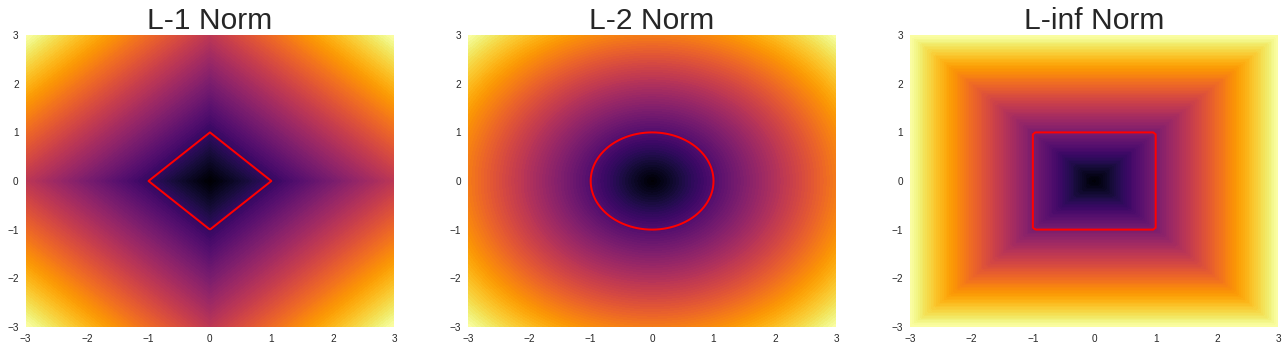
\includegraphics[width=0.8\textwidth]{norm.png}  
	                % reference folder/figure.pdf here and adjust width
	        \captionsetup{labelformat=empty}
	        \caption{}
	        \label{fig:my_label}
	    \end{figure}
	\end{soln}
\end{enumerate}




\subsection{Geometry}
Prove that these are true or false. Provide all steps.
\begin{enumerate}
\item 	The smallest Euclidean distance from the origin to some point $\mathbf{x}$ in the hyperplane $\mathbf{w}^T\mathbf{x} + b = 0$ is $\frac{|b|}{||\mathbf{w}||_2}$.\\
\begin{soln}  
	Suppose we find a point $X$ on the hyperplane. We essentially need to find the projection of the vector from $X$ to $X_0(0,0)$ on the perpendicular to the hyperplane $\mathbf{w}^T\mathbf{x} + b = 0$. We know that the perpendicular to the hyperplane $\mathbf{w}^T\mathbf{x} + b = 0$ is $\mathbf{w}$. Thus, \\
	
	d = projection of $X-X_0$ on $\mathbf{w}$\\
	
	Let $(X - X_0) = a$
	
	$d = ||a||_2 cos \theta = ||a||_2 \frac{w a}{||a||_2 ||w||_2}  = \frac{w a}{||w||_2}$ \\
	
	Substituting $a = (X - X_0)$ \\
	
	$d = \frac{w \dot (X - X_0)}{||w||_2} = \frac{w^TX - w^TX_0}{||w||_2} = \frac{|b|}{||w||_2}$
	 
	
	%d =  $ || \frac{(X - X_0) \dot w }{w \dot w} w || = \frac{X \dot w - X_0 \dot w}{||w||} = \frac{|b| - 0}{||w||}$ = $\frac{|b|}{||w||_2}$ 
	
	
\end{soln}

\item 	The Euclidean distance between two parallel hyperplane $\mathbf{w}^T\mathbf{x} + b_1 = 0$ and $\mathbf{w}^T\mathbf{x} + b_2 = 0$ is $\frac{|b_1 - b_2|}{||\mathbf{w}||_2}$ (Hint: you can use the result from the last question to help you prove this one).

\begin{soln}  We can find the distances $d_1$ and $d_2$ for both the hyperplanes respectively and notice that our final solution $d = d_1 - d_2$. \\
$$
d1 = \frac{|b_1|}{||w||_2} \\
d2 = \frac{|b_1|}{||w||_2} \\ 
d = d1 - d2 = \frac{|b_1 - b_2|}{||\mathbf{w}||_2}
$$ \end{soln}

\end{enumerate}



\section{Programming Skills - Matlab [5pts]}
Sampling from a distribution.  For each question, submit a scatter plot (you will have 5 plots in total).  Make sure the axes for all plots have the same limits.  (Hint: You can save a Matlab figure as a pdf, and then use includegraphics to include the pdf in your latex file.)
\begin{enumerate}
\item Draw 100 samples $\mathbf{x} = [x_1, x_2]^T$ from a
  2-dimensional Gaussian distribution with mean $(0, 0)^T$ and
  identity covariance matrix, i.e.,
  $p(\mathbf{x}) =
  \frac{1}{2\pi}\exp\left(-\frac{||\mathbf{x}||^2}{2}\right)$, and
  make a scatter plot ($x_1$ vs. $x_2$).  For each question below, make each change separately to
  this distribution.
  
	\begin{soln}
	    Points centred around [0,0].
	    \begin{figure}[H]
	        \centering
	        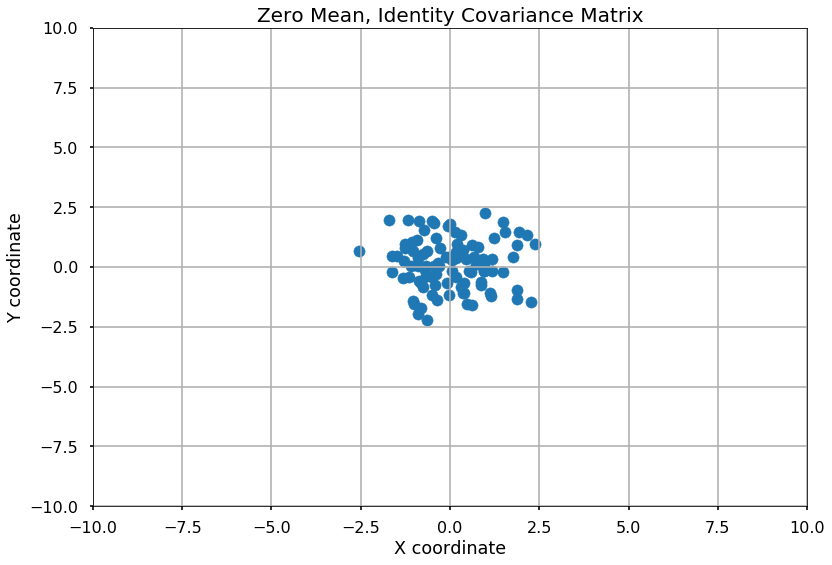
\includegraphics[width=0.65\textwidth]{1.png}
	        \captionsetup{labelformat=empty}
	        \caption{}
	        \label{fig:my_label}
	    \end{figure}
	\end{soln}
\item Make a scatter plot with a changed mean of $(1, -1)^T$.\\
	\begin{soln}
	    Same as before, but points are now centered around [1,-1]
	    \begin{figure}[H]
	        \centering
	        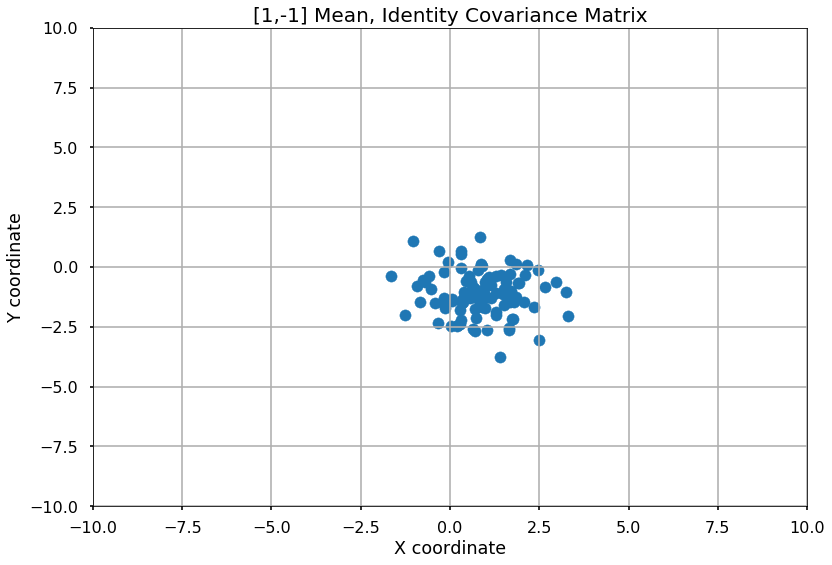
\includegraphics[width=0.65\textwidth]{2.png}
	        \captionsetup{labelformat=empty}
	        \caption{}
	        \label{fig:my_label}
	    \end{figure}
	\end{soln}
\item Make a scatter plot with a changed covariance matrix of $\begin{pmatrix}
    2 & 0 \\ 0 & 2\\
  \end{pmatrix}$.\\
  	\begin{soln}
  	    Same as 1, but doubled spread or variance across both dimensions.
	    \begin{figure}[H]
	        \centering
	        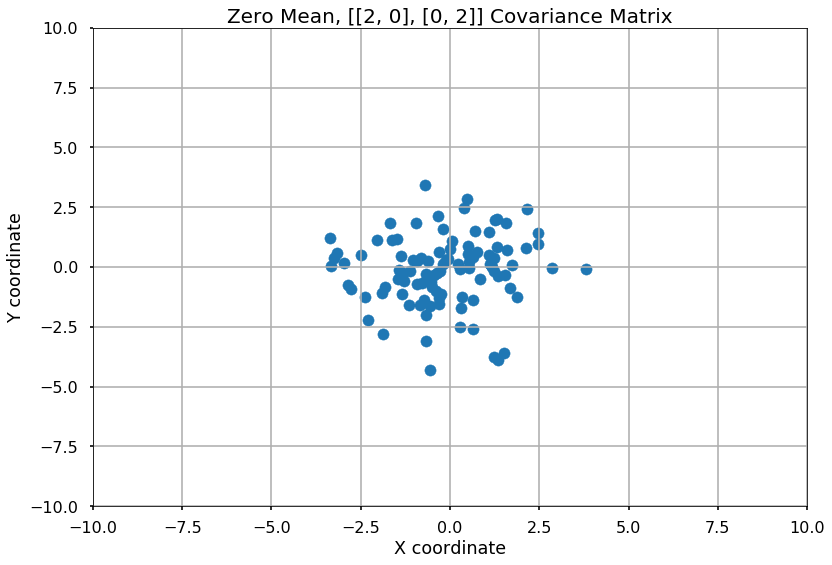
\includegraphics[width=0.65\textwidth]{3.png}
	        \captionsetup{labelformat=empty}
	        \caption{}
	        \label{fig:my_label}
	    \end{figure}
	\end{soln}
\item Make a scatter plot with a changed covariance matrix of $\begin{pmatrix}
    2 & 0.2 \\ 0.2 & 2\\
  \end{pmatrix}$.\\
  	\begin{soln}
  	    Same as 4, but there's a small positive correlation with x1 and x2.
	    \begin{figure}[H]
	        \centering
	        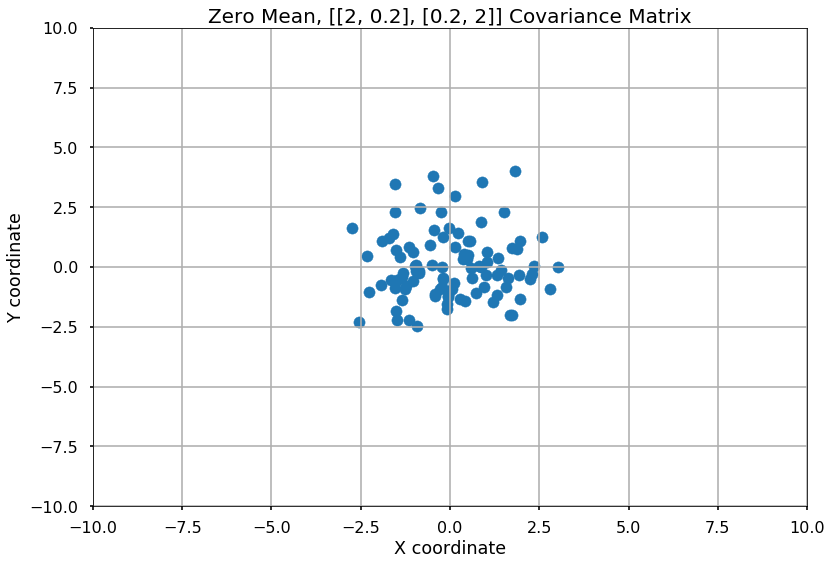
\includegraphics[width=0.65\textwidth]{4.png}
	        \captionsetup{labelformat=empty}
	        \caption{}
	        \label{fig:my_label}
	    \end{figure}
	\end{soln}
\item Make a scatter plot with a changed covariance matrix of $\begin{pmatrix}
    2 & -0.2 \\ -0.2 & 2\\
  \end{pmatrix}$.	\\
  	\begin{soln}
  	    Same as 4, but there's a small negative correlation with x1 and x2.
	    \begin{figure}[H]
	        \centering
	        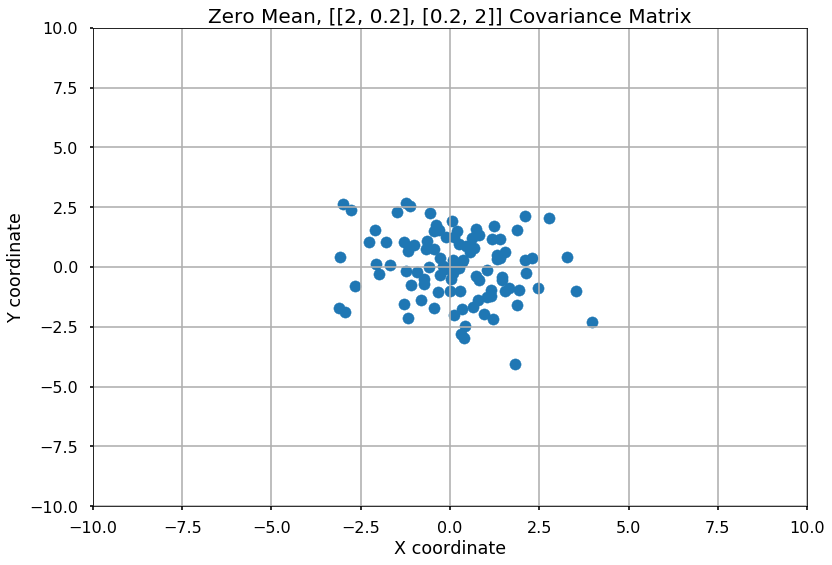
\includegraphics[width=0.65\textwidth]{5.png}
	        \captionsetup{labelformat=empty}
	        \caption{}
	        \label{fig:my_label}
	    \end{figure}
	\end{soln}
\end{enumerate}


\bibliographystyle{apalike}


%----------------------------------------------------------------------------------------


\end{document}
